\section{ Introduction }
\subsection{ Imitation of Instruments }
Let’s not mention the old greeks, german yodeling, or the lullabies of our mothers, but instead start from the modern utilization of musical instruments and rhythmic compositions. In the modern ages people have had the need to imitate instruments for several reasons. One is to describe melodies, rhytms, tones and feelings in the creation of music to others. Another reason could be the lack of instruments while still wanting to socially interact with others and to perform complex instrumental patterns vocally. Lastly simply because we as human beings get songs in our heads and intuitively burst out into humming and imitating music we’ve heard because we can’t stop it. One can say that we have had the need to imitate instrumental sounds since the invention of music.
\subsection{ Vocal Percussion }
Using mouth, lips and throat to produce percussion sounds and effects is seen in many cultures all through history. North American scat singing, African Khoisan i.e. Click Language (e.g. Xhosa from South Africa and Khoekhoe from Botswana) are among the cultural examples (Choi, 2013).	
The modern day equivalent is known as Beatboxing which is primarily linked to the early hip-hop-culture in the 1980’ies. The self-proclaimed pioneer of Beatboxing, Doug E. Fresh also known as ‘The Human Beatbox’ was a key player in making Beatboxing famous. However, other earlier artists has been known to use similar techniques of vocal percussion in published material e.g. Paul McCartney with the song “That Would Be Something” from 1969.
\subsection{ Beatboxing }
Human Beatboxing is generally limited to percussive sounds produced by the vocal cord and body (e.g. clapping) to imitate rhythms of a drumset i.e. snare drum, hi-hat, kick drums, cymbals etc. but some Beatboxers also imitates bass and guitar and occasionally combined with vocal. An example of this is Michael Winslow, an American comedian, actor, and beatboxer probably best known for his ability to make realistic sound effects with his voice in the movie Police Academy (1984). Beatboxing as an artform was an outspring of the hip hop culture since the 1980’ies. It was shaped by musical technologies in context with its age, and through time it evolved to become a complex instrumental expression. In the origin of human beatboxing it was meant to imitate grooves and beats but soon it utilized sounds like basslines, scratching, effects, noise, and almost every musical instrument and “filters”. –With improved techniques and sophisticated microphone technology beatboxing became a modern instrumental element in many music genres of today.
\subsection{ Software to transcribe instruments }
Since “modern beatboxing” evolved, it seems like technology is reclaiming it’s technological importance. Some artists are beginning to transcribe instruments, adding filters and effects to beatboxing which takes the complexity of beatboxing even further. I.e. Dub FX, Benjamin Stanford from Australia, who samples sequences of vocal basslines, grooves and adds effects to them. Lately he re-recorded ‘Love Someone’ using Roland RC-505, a so called ‘Loop Station’, based on sequential recording of each track in instrumental compositions. [2] This way, he can perform on streets as one person, sounding as an orchestra. ** NEED TO WRITE MORE ON TRANSCRiPTION**
\\
\begin{figure}[h]
	\begin{center}
		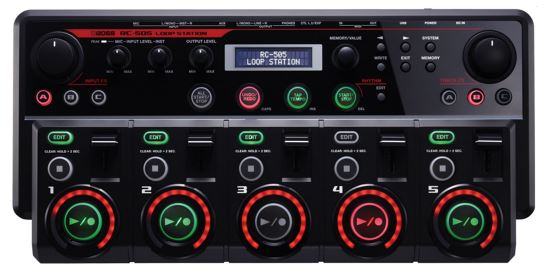
\includegraphics[height=5cm]{fig/Roland-RC-505.JPG}
		\caption{Roland Looper RC-505}
		\label{Looper}
	\end{center}
\end{figure}
\\
\subsection{ Motivation }
The motivation of this project is the admiration of innovative artforms and to explore the opportunities that arise from them. It is the fact that any analog instrument can be treated as a source for digital and electronic processing. Paradoxically beatboxing comes from imitating other analog instruments, but every other analog instrument is also victimized by digitalization. Jimi Hendrix pushed the creative scope of playing guitar, Jean Michel Jarre by playing piano and electronic drums. Why shouldn’t beatboxing be treated as an analog instrument as well? 
\subsection{ Why Beatboxing? }
The good thing about beatboxing is that it is under constant adaption to modern instrument technologies. It’s intuitively the fast way forward to learn grooves and rhythms. Beatboxing comes easy to many even though it requires one to let go of shyness, -like any other instrument. The good thing about beatboxing is that it comes relatively easy to many people. It only requires creativity to imitate sounds and instruments, while many people also tends to have the ability of humming with decent outcome. If technology can provide additional possibilities to facilitate the creation music that sounds good, it can be a fun way to learn the principles of rhythm and to produce satisfactory music, even that one does not know the basics or the techniques of a traditional instrument. 